\documentclass[WHATMANUAL.tex]{subfiles}

\begin{document}

\chapter[Hydrogeological characterization of the confinement conditions of the regional bedrock aquifer in Monteregie Est]{Hydrogeological characterization of the confinement conditions of the regional bedrock aquifer in Monteregie Est\footnotemark}\label{app:confinement_cond_in_MontEst}

\footnotetext{This work has been produced with the participation of Dr. René Lefebvre at INRS-ETE, 490 rue de la Couronne, Quebec City, Quebec, Canada.}

The water level was monitored in 44 observation wells during the PACES project in Monteregie Est for a period of approximately two years. The vast majority of the wells were installed in the regional fractured bedrock aquifer. Daily weather data for 32 weather stations in and around the Monteregie Est area were also retrieved from the Canadian Daily Climate Database (CDCD) with the software WHAT for the years 2000 to 2012. Missing values in the weather time series were also estimated with WHAT to produce gapless meteorological records of daily air temperature and precipitation.
 
Thiessen polygons were generated from the location of the 32 weather stations (see Figure~\ref{fig:Thiessen_meteo_wells}). The hydrographs were next produced with WHAT by selecting the weather data on the basis of these polygons. These hydrographs were then inspected visually and grouped into three different classes according to their relative behavior to precipitation and snow melt events. These classes are interpreted in terms of confinement conditions of the regional bedrock aquifer: (1) unconfined, (2) confined, and (3) semi-confined or confined with regional influences from a nearby recharging zone. The containment conditions of the regional bedrock aquifer have been thus deducted at 35 sites in total since a number of the 44 wells are multi-level and are located side by side at the same location. Figure~\ref{fig:casTypes_hydrographs} shows typical hydrograph relating to the various conditions of confinement.

\begin{figure}[!ht]
\centering
\includegraphics[width=0.75\textwidth]{img/Thiessen_meteo_wells}
\caption[Locations of observation wells (green dots) and weather stations (blackheads) in the Monteregie Est area.]{Locations of observation wells (green dots) and weather stations (blackheads) in the Monteregie Est area.}
\label{fig:Thiessen_meteo_wells}
\end{figure}

The confinement conditions deducted from the well hydrographs were drawn on the map of confinement conditions of the regional bedrock aquifer which was produced based on the sequence and thickness of the surficial deposits \citep{carrier_portrait_2013}. These results show that a simple qualitative visual interpretation of the well hydrographs can provide an independent validation of the criteria used to define the confinement conditions of the regional bedrock aquifer.

Figure 3 shows that the confinement conditions of the regional bedrock aquifer defined on the basis of well hydrographs are generally consistent with those of the map of confinement conditions. This is an interesting result since the two approaches are independent. That is, the definition contained conditions of bedrock aquifer for both approaches stems criteria based on physical quantities that are very different in nature: time series of groundwater levels in one case and spatial distribution of surficial deposits in the other. The confinement conditions deduced from the well hydrographs come and validate the criteria used to produce the regional map contained conditions. These criteria were based on professional judgment and are therefore relatively arbitrary, even if they are logical according to regional conditions.

\begin{figure}[!hb]
\centering
\includegraphics[width=0.75\textwidth]{img/CasTypes.png}
\caption[Typical hydrographs relating to the three classes that were considered in the analysis of the confinement conditions of the regional bedrock aquifer in the Monteregie Est area, Quebec, Canada.]{Typical hydrographs relating to the three classes that were considered in the analysis of the confinement conditions of the regional bedrock aquifer in the Monteregie Est area, Quebec, Canada: (top) confined, (middle) semi-confined or confined with regional influences, and (bottom) unconfined.}
\label{fig:casTypes_hydrographs}
\end{figure}

\begin{figure}
\centering
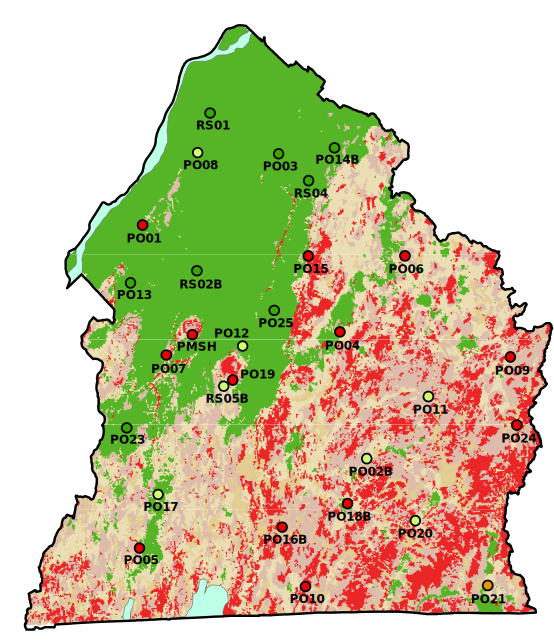
\includegraphics[height=0.85\textheight]{img/CONFINEMENTetPUITS}
\caption[Confinement conditions deducted from the well hydrographs compared to the map of confinement conditions of the regional bedrock aquifer.]{Confinement conditions deducted from the well hydrographs (dots) compared to the map of confinement conditions of the regional bedrock aquifer. The colors indicate the conditions of confinement of the aquifer, both for the map and the well symbols: green for captive, red for free, and other tones for semi-captive.}
\label{fig:tab_hydrograph_layout}
\end{figure}

De façon globale, les résultats obtenus avec les hydrogrammes de puits sont également cohérents avec les différents contextes hydrogéologiques définis en Montérégie Est. On retrouve les puits d’observation jugés représentatifs de conditions captives exclusivement dans les Basses-terres, principalement dans la partie nord de la région où on retrouve une grande épaisseur d’argile. De plus, les hydrogrammes donnent des indications du confinement pour des zones plus locales. Par exemple, le puits PO01 représente bien la zone de recharge locale située dans la partie nord-ouest des Basses-terres, où l'on retrouve des dépôts meubles moins épais et ayant une texture plus grossière. On note également que le puits PO08, situé à environ 20 km de PO01 et à moins de 7 km de la limite de cette zone de recharge, présente des variations saisonnières de la piézométrie qui sont importantes (de 1 à 2 m de 2010 à 2012) en dépit de l'épaisse couche d'argile (plus de 25 m) qui recouvre le roc à cet endroit. Il est possible que ces variations du niveau piézométrique au puits PO08 soient causées par une influence provenant de la zone de recharge du roc située à proximité. La partie sud des Basses-terres est caractérisée quant à elle par des puits reflétant des conditions captives, semi-captives et libres qui sont distribuées de façon cohérente avec la carte des conditions de confinement.

Le Piémont appalachien est caractérisé par des puits indiquant exclusivement des conditions libres. Plus spécifiquement, le puits PO18 situé dans une petite cuvette du roc dans le sud du Piémont est particulièrement intéressant. Malgré que le roc soit recouvert de plus de 40 m de dépôts meubles à cet endroit, on observe que les variations du niveau d'eau dans le puits sont fortement corrélées avec les précipitations et la fonte printanière, indiquant des conditions libres. Ceci suggère que l'aquifère rocheux régional dans la cuvette est fortement connecté à l'aquifère rocheux libre à semi-captif retrouvé tout autour de la cuvette. Il est intéressant de voir comment il est possible d'utiliser la carte de confinement  du roc comme un outil pour expliquer le comportement de la piézométrie mesurée dans les puits d'observation.

Les Hautes-terres appalachiennes sont caractérisées par des puits indiquant des conditions allant de libres à semi-captives. Ces résultats représentent bien la couverture discontinue des dépôts meubles dans ce contexte hydrogéologique. Le fait que l'on ne retrouve pas de puits indiquant des conditions captives, malgré des épaisseurs de dépôts meubles parfois importantes dans les vallées, incluant des sédiments fins, suggère une influence significative des zones de recharge de l’aquifère rocheux situées en élévation sur les zones située dans les creux topographiques (vallées). Le puits PO20, classé comme ayant un comportement de type semi-captif et montrant plus de 24 m de dépôts, est un bon exemple.

Les puits localisés sur ou près des Montérégiennes représentent également bien ce que l'on retrouve sur la carte des conditions de confinement de l’aquifère rocheux régional. On remarque que les puits indiquent des conditions libres sur les Montérégiennes et des conditions qui varient entre libres et semi-captives au pourtour de celles-ci. Cela est particulièrement bien représenté par les puits PO19, PO12 et RS05b situés dans les environs du Mont Rougemont : le puits PO19, situé directement sur le Mont Rougemont, indique des conditions libres, alors que les puits PO12 et RS05b ont une réponse indiquant des conditions semi-captives. Ce comportement est particulièrement surprenant pour le puits PO12 où le roc est recouvert par une épaisse couche de silt argileux de plus de 23 m. Ceci pourrait être un indicateur de l'étendue de l'influence de la recharge de l’aquifère rocheux par les Montérégiennes. Ces collines sont effectivement considérées comme étant des zones de recharge préférentielle dans la région et ces données semblent suggérer qu’elles pourraient même avoir une influence sur la piézométrie de l’aquifère rocheux à une certaine distance des Montérégiennes, où l’aquifère rocheux peut être recouvert par d'importantes épaisseurs de sédiments fins.

L'interprétation qualitative de la réponse des niveaux d'eau aux événements de précipitations et de fonte de la neige a permis de valider l’évaluation des conditions de confinement basée sur l’épaisseur et la nature des dépôts meubles. 

Because detailed information about the spatial distribution of the unconsolidated sediment is not common to every project in hydrogeology.

Actually the containment level of the bedrock aquifer is not clearly defined into three distinct classes, but varies over a continuous range of conditions ranging from perfectly free to completely confined. The classification of the well is even more difficult considering the relatively short period (2 years or less) on which water level data are currently available for the majority of the wells. A complementary analysis would be the calculation of the barometric response function of the well using measurement of water level and atmosphéric pressure with a high temporal resolution (4 measurements per hour). The application of this approach to the data acquired in the Monterie Est area is presented in Appenx~X.

\end{document}